
\section{enzymes.xml}

The enzyme file is used to define enzyme composition and efficiency.
It defines efficiency constraints in the RBA model.
These constraints ensure that a reaction flux is smaller than
the producf of efficiency and concentration of the enzyme catalyzing
the reaction.

\subsection{RBAEnzymes}
\label{sec:rba_enzymes}

The outermost portion of the metabolism file is an instance of class
\rbaenzymes, shown in Figure~\ref{fig:enzymes_doc}.

\begin{figure}
  \centering
  \includegraphics[scale=0.8]{figures/enzymes_doc}
  \caption{XML structure of enzyme document.}
\label{fig:enzymes_doc}
\end{figure}

\rbaenzymes{} has no simple attributes.

It contains exactly one instance of \textbf{ListOfEfficiencyFunctions}.
This list contains \function{} definitions \emph{without} a
\textbf{ListOfParameter}.
The variable of the \function{}s is the growth rate.
These functions can be used to define different
\emph{sets} of efficiency functions.
A classical application is to define one function per external medium.
Suppose the function identifiers are
\textbf{medium\_1}, \ldots, \textbf{medium\_N}.
Every \enzyme{} must redefine these functions and associate enzyme-specific
parameters.
For example, for enzyme A, parameters for function \textbf{medium\_1}
will reflect the efficiency of A in the first medium.
This structure allows to solve RBA for different sets of enzyme
efficiencies.

It contains excatly one instance of \textbf{ListOfEnzymes} that is used
to store \enzyme{} information.


\subsection{Enzyme}
\label{sec:enzyme}

The \enzyme{} class is used to define enzymes
(Fig.~\ref{fig:enzymes_enzyme}).

\begin{figure}
  \centering
  \includegraphics[scale=0.8]{figures/enzymes_enzyme}
  \caption{Class storing enzyme information.}
\label{fig:enzymes_enzyme}
\end{figure}

It contains a \machinerycomposition{} that refers to metabolic \species{}
and \macromolecule{}s composing the \enzyme{}.
Note that the composition can be left unspecified.
In this case, the reaction associated with the enzyme is considered spontaneous.

It contains an \enzymaticactivity{} instance that is used to specify
the various \enzymeefficiency{} functions.
It also contains transporter activity information (if applicable).

\paragraph{The \textit{id} attribute}
The \textbf{id} attribute is a string defining the identifier of
the enzyme.

\paragraph{The \textit{zeroCost} attribute}
The \textbf{zeroCost} attribute is a boolean value.
If set to true, the reaction associated may occur without having to produce
the enzyme.
If set to false or unspecified, an efficiency constraint is created where the
flux through the reaction has to be smaller than the product of enzyme
efficiency and enzyme concentration.


\subsection{EnzymaticActivity}
\label{sec:enzymatic_activity}

The \enzymaticactivity{} class is used to store information about
enzyme efficiency and transporter efficiency (Fig.~\ref{fig:enzymes_enzyme}).

It contains one instance of \textbf{ListOfEnzymeEfficiencies}.
This list redefines the efficiency functions in \rbaenzymes{}
with parameters specific to an enzyme.

It contains one instance of \textbf{ListOfFunctions} representing
transporter efficiency.
Each \function{} in the list must specify a \textbf{variable} attribute.
The \textbf{variable} attribute is the metabolite whose external concentration
affects the transport rate (usually the chemical imported or a cofactor).
The transport efficiency is computed by \emph{multiplying} the results
of all the functions listed.
Note that the transport efficiency can depend on an arbitrary number of
chemicals.

\paragraph{The \textit{reaction} attribute}
The \textbf{reaction} attribute must match the identifier of a metabolic
\reaction.
This is a one-to-one mapping.
A \reaction{} can only have one associated \enzyme{}.
If several \enzyme{}s catalyze the same \reaction{},
the \reaction{} must be duplicated.


\subsection{EnzymeEfficiency}
\label{sec:enzyme_efficiency}

The \enzymeefficiency{} class is used to define parameters
for an efficiency function (Fig.~\ref{fig:enzymes_enzyme}).
It contains one instance of \textbf{ListOfParameters}.
The \parameter{}s must match the type of the efficiency function
(as specified in the \rbaenzymes{} instance) being redefined.

\paragraph{The \textit{function} attribute}
The \textbf{function} attribute must match the identifier of an efficiency
function defined in the same \rbaenzymes{} instance.
